% $Header: /cvsroot/latex-beamer/latex-beamer/solutions/conference-talks/conference-ornate-20min.en.tex,v 1.6 2004/10/07 20:53:08 tantau Exp $

\documentclass[11pt]{beamer}

% This file is a solution template for:

% - Talk at a conference/colloquium.
% - Talk length is about 20min.
% - Style is ornate.

% Copyright 2004 by Till Tantau <tantau@users.sourceforge.net>.
%
% In principle, this file can be redistributed and/or modified under
% the terms of the GNU Public License, version 2.
%
% However, this file is supposed to be a template to be modified
% for your own needs. For this reason, if you use this file as a
% template and not specifically distribute it as part of a another
% package/program, I grant the extra permission to freely copy and
% modify this file as you see fit and even to delete this copyright
% notice. 


\mode<presentation>
{
  % Turn off shadowing, large frame titles, and sans-serif fonts
  % (ALL OF WHICH PISS ME OFF - RBN).
  \usetheme{default}
  \usefonttheme{serif}
  \usecolortheme[RGB={0,0,0}]{structure}
  \setbeamercovered{transparent}
  \setbeamerfont{frametitle}{size=\normalsize,series=\bfseries}
}

\usepackage{graphics}

\usepackage[english]{babel}
% or whatever

%\usepackage[latin1]{inputenc}
% or whatever

\usepackage{times}
\usepackage[T1]{fontenc}
% Or whatever. Note that the encoding and the font should match. If T1
% does not look nice, try deleting the line with the fontenc.

% Add a frame indication to the navigation symbols
\setbeamertemplate{navigation symbols}{}
\setbeamertemplate{footline}{
\vskip1mm \ 
{\it \insertshorttitle}
\hfill
Frame \insertframenumber\ of \inserttotalframenumber\ 
\insertslidenavigationsymbol
\insertframenavigationsymbol
\insertsubsectionnavigationsymbol
\insertsectionnavigationsymbol
\insertdocnavigationsymbol
\insertbackfindforwardnavigationsymbol
\  \vskip1mm
}

\setbeamertemplate{bibliography item}[text]{}

\title[Scenario comparisons: How much good can we do?] % (optional, use only with long paper titles)
{

\includegraphics[height=1cm]{imperial.pdf}\hfill
\includegraphics[height=1.6cm]{ga2len_logo.pdf}\\
\textbf{Scenario comparisons: How much good can we do?}
}

\author[Author, Another] % (optional, use only with lots of authors)
% {F.~Author\inst{1} \and S.~Another\inst{2}}
{
Roger B. Newson
\\ \href{mailto:r.newson@imperial.ac.uk}{r.newson@imperial.ac.uk}
\\ \href{http://www.imperial.ac.uk/nhli/r.newson/}{\textsl{http://www.imperial.ac.uk/nhli/r.newson/}}
}
% - Give the names in the same order as the appear in the paper.
% - Use the \inst{?} command only if the authors have different
%   affiliation.

%\institute[Universities of Somewhere and Elsewhere] % (optional, but mostly needed)
\institute[Imperial College London]
{
Imperial College London\\
}
\date[UKSUG 2012] % (optional, should be abbreviation of conference name)
{
Updated from the 18th UK Stata Users' Group Meeting, 13--14~September, 2012
\\ Original version downloadable from the conference website at
\\ \href{http://ideas.repec.org/s/boc/usug12.html}{\textsl{http://ideas.repec.org/s/boc/usug12.html}}
}


\subject{Statistics}
% This is only inserted into the PDF information catalog. Can be left
% out. 


% If you have a file called "university-logo-filename.xxx", where xxx
% is a graphic format that can be processed by latex or pdflatex,
% resp., then you can add a logo as follows:

% \pgfdeclareimage[height=0.5cm]{university-logo}{university-logo-filename}
% \logo{\pgfuseimage{university-logo}}

% \pgfdeclareimage[height=0.5cm]{university-logo}{imperial.pdf}
% \logo{\pgfuseimage{university-logo}}


\begin{document}

\section{Title}

\begin{frame}
  \titlepage
\end{frame}

\section{Introduction}

%\begin{frame}
%  \frametitle{Outline}
%  \tableofcontents[pausesections]
%  % You might wish to add the option [pausesections]
%\end{frame}

\begin{frame}
\frametitle{What are scenario comparisons?}

\begin{itemize}

\item<2-> Applied scientists, especially public health scientists, frequently want to know how much good can be caused
by a proposed intervention.

\item<3-> \textit{For instance}, we might want to estimate how much we could decrease the level
of a disease, in a dream scenario where the whole world stopped smoking.

\item<4-> In statistics, scenarios are different versions of a dataset,
with the same variables but different values and/or observations.

\item<5-> We may want to compare different scenarios applied to the same population
(with the same parameters).

\item<6-> Alternatively, we may want to compare the same scenario between different populations
(with different parameters),
as when standardizing disease rates to a common distribution of gender and age.

\item<7-> Scenario comparison statistics include pairwise comparisons,
population attributable risks and fractions,
and age--standardized heterogeneity chi--squared tests.

\end{itemize}

\end{frame}

\begin{frame}
\frametitle{Existing Stata tools for scenario comparisons}

\begin{itemize}

\item<2-> Brady (1998)\cite{brady1998} introduced the Stata Version~5 package \texttt{aflogit}
for estimating the population attributable fraction (with confidence limits) for cohort and case--control data.

\item<3-> This is still used, although it sometimes has problems with the 32--character names
used in later Stata versions.

\item<4-> In Stata Version~11, the \texttt{margins} command was added,
allowing estimation (with confidence limits) of scenario means of a wide range of quantities.

\item<5-> In Stata Version~12, the \texttt{pwcompare} command was added,
together with the \texttt{pwcompare} option of \texttt{margins},
to estimate pairwise differences between scenario means.

\item<6-> These new tools are very comprehensive,
allowing the use of sample survey data,
and the use of the Shah variance\cite{shah2004} to estimate confidence limits.

\end{itemize}

\end{frame}

\section{The \texttt{punaf} suite of packages}

\begin{frame}
\frametitle{The \texttt{punaf} suite of packages}

\begin{itemize}

\item<2-> The \texttt{punaf} suite of packages (Newson, 2013)\cite{newson2013} can be downloaded from SSC,
and includes \texttt{punaf}, \texttt{punafcc}, \texttt{regpar}, \texttt{margprev}, \texttt{marglmean},
and now \texttt{scenttest}.

\item<3-> They use \texttt{margins} to compute confidence intervals
for scenario means and proportions and/or their comparisons
(differences and ratios),
including population attributable (and unattributable) risks and fractions.

\item<4-> These are estimated (using \texttt{nlcom}) with asymmetric confidence limits,
calculated from appropriate Normalizing and variance--stabilizing transformations.

\item<5-> The results may be saved as estimation results,
and/or listed, and/or saved in output datasets,
using the SSC package \texttt{parmest}.

\end{itemize}

\end{frame}

\begin{frame}
\frametitle{Packages of the \texttt{punaf} suite}

These estimate and/or compare marginal means and/or prevalences for one and/or two scenarios
(``Scenario 1'' and ``Scenario 0''),
using Normalizing and variance--stabilizing transformations.

{\scriptsize

\begin{center}
\begin{tabular}{rp{50mm}l}
\hline
\textit{Package}&\textit{Computes confidence intervals for:}&\textit{Transformation}\\
\hline
\texttt{margprev}&Marginal prevalences&Logit\\
\texttt{marglmean}&Marginal arithmetic means&Log\\
\texttt{regpar}&Differences between marginal prevalences (population attributable risks (PARs))&Fisher's $z$\\
\texttt{punaf}&Ratios between marginal arithmetic means (population unattributable fractions (PUFs))&Log\\
\texttt{punafcc}&Arithmetic mean risk or hazard ratios (case--control or survival PUFs)&Log\\
\texttt{scenttest}&Differences between marginal arithmetic means, or between marginal Poisson rates (PARs)&Identity\\
\hline
\end{tabular}
\end{center}

}

A population \textit{attributable} fraction (PAF) is estimated by end--point transformation,
subtracting the corresponding PUF from 1,
as recommended by Greenland and Drescher (1993)\cite{greenland1993}.

\end{frame}

\section{Examples in the \texttt{lbw} data}

\begin{frame}
\frametitle{Examples in the \texttt{lbw} data}

\begin{itemize}

\item<2-> The \texttt{lbw} dataset was discussed by Hosmer, Lemeshow and Klar (1988)\cite{hosmer1988},
and is distributed on--line by Stata Press.

\item<3-> It has one observation for each of a sample of
189 pregnancies, and data on the birth weight of the baby,
and on a list of predictive variables.

\item<4-> The most interesting of these variables is probably the mother's smoking status during pregnancy,
coded as the binary variable \texttt{smoke}.

\item<5-> In our examples,
we will try to estimate how much good could be done by eliminating smoking (at least during pregnancy).

\item<6-> This good is measured using scenario prevalences of low birth weight,
which is stored in the binary variable \texttt{low}
(birth weight below 2500 grams).

\end{itemize}

\end{frame}

\begin{frame}[fragile]
\frametitle{Logistic regression in the \texttt{lbw} data}

After loading the \texttt{lbw} data, we fit a logistic regression model of \texttt{low}
with respect to \texttt{smoke} and the confounder \texttt{race}
(white, black or other):

\tiny
\begin{verbatim}
. logit low i.race i.smoke, or vce(robust);

Iteration 0:   log pseudolikelihood =   -117.336  
Iteration 1:   log pseudolikelihood = -110.10441  
Iteration 2:   log pseudolikelihood = -109.98749  
Iteration 3:   log pseudolikelihood = -109.98736  
Iteration 4:   log pseudolikelihood = -109.98736  

Logistic regression                               Number of obs   =        189
                                                  Wald chi2(3)    =      14.30
                                                  Prob > chi2     =     0.0025
Log pseudolikelihood = -109.98736                 Pseudo R2       =     0.0626

------------------------------------------------------------------------------
             |               Robust
         low | Odds Ratio   Std. Err.      z    P>|z|     [95% Conf. Interval]
-------------+----------------------------------------------------------------
        race |
      black  |   2.956742   1.420439     2.26   0.024     1.153162    7.581175
      other  |   3.030001   1.187272     2.83   0.005     1.405753    6.530954
             |
     1.smoke |   3.052631    1.10296     3.09   0.002     1.503568    6.197631
       _cons |   .1587319   .0515235    -5.67   0.000     .0840173    .2998882
------------------------------------------------------------------------------
\end{verbatim}
\normalsize

We see that maternal smoking trebles the odds of low birth weight.

\end{frame}

\begin{frame}
\frametitle{But how much good can we do?}

\begin{itemize}

\item<2-> Not many people really understand odds ratios.

\item<3-> An audience of non--mathematicians might prefer to know what difference it would make,
if all pregnant mothers stopped smoking.

\item<4-> The \texttt{regpar} package can answer this question,
by comparing prevalences of low birth rate under 2 scenarios.

\item<5-> ``Scenario 0'' is the world we live in, where some mothers smoke.

\item<6-> ``Scenario 1'' is a fantasy world, where no mothers smoke,
but the race distribution stays the same.

\item<7-> The difference between these prevalences is the \textbf{population attributable risk (PAR)}.

\end{itemize}

\end{frame}

\begin{frame}[fragile]
\frametitle{Scenario prevalences and the PAR using \texttt{regpar}}

We execute \texttt{regpar}, as follows:

\tiny
\begin{verbatim}
. regpar, at(smoke=0);
Scenario 0: (asobserved) _all
Scenario 1: smoke=0
Symmetric confidence intervals for the logit proportions
under Scenario 0 and Scenario 1
and for the z-transformed population attributable risk (PAR)
Total number of observations used: 189
------------------------------------------------------------------------------
             |      Coef.   Std. Err.      z    P>|z|     [95% Conf. Interval]
-------------+----------------------------------------------------------------
  Scenario_0 |   -.789997   .1519305    -5.20   0.000    -1.087775   -.4922187
  Scenario_1 |  -1.215955   .2051031    -5.93   0.000     -1.61795   -.8139606
         PAR |   .0837153   .0266196     3.14   0.002     .0315419    .1358887
------------------------------------------------------------------------------

Asymmetric 95% CIs for the untransformed proportions
under Scenario 0 and Scenario 1
and for the untransformed population attributable risk (PAR)
               Estimate    Minimum    Maximum 
  Scenario_0   .3121693   .2520374    .379371 
  Scenario_1    .228649   .1654878   .3070471 
         PAR   .0835203   .0315315   .1350584 
\end{verbatim}
\normalsize

We see that 3.2 to 13.5 percent of all babies might be saved from low birth weight,
if no mothers smoked.

\end{frame}

\begin{frame}
\frametitle{Advice for smoking mothers}

\begin{itemize}

\item<2-> Our \textit{real} aim is to communicate our message to an audience of smoking mothers,
and not just to an audience of target--minded public health professionals.

\item<3-> This non--professional audience might want to know what good \textit{they} could do
for \textit{their} babies.

\item<4-> The \texttt{regpar} package can answer this question, too,
by comparing prevalences of low birth weight under the 2 scenarios
\textit{in the subpopulation of smoking mothers}.

\item<5-> This is done using the \texttt{subpop()} option of \texttt{regpar}.

\end{itemize}

\end{frame}

\begin{frame}[fragile]
\frametitle{Scenario prevalences and the exposed subpopulation attributable risk for smoking mothers}

We execute \texttt{regpar} with the \texttt{subpop()} option:

\tiny
\begin{verbatim}
. regpar, at(smoke=0) subpop(if smoke==1);
Scenario 0: (asobserved) _all
Scenario 1: smoke=0
Symmetric confidence intervals for the logit proportions
under Scenario 0 and Scenario 1
and for the z-transformed population attributable risk (PAR)
Total number of observations used: 189
------------------------------------------------------------------------------
             |      Coef.   Std. Err.      z    P>|z|     [95% Conf. Interval]
-------------+----------------------------------------------------------------
  Scenario_0 |  -.3829923   .2373852    -1.61   0.107    -.8482587    .0822742
  Scenario_1 |  -1.436486   .2279922    -6.30   0.000    -1.883343   -.9896299
         PAR |   .2166422   .0707321     3.06   0.002     .0780098    .3552746
------------------------------------------------------------------------------

Asymmetric 95% CIs for the untransformed proportions
under Scenario 0 and Scenario 1
and for the untransformed population attributable risk (PAR)
               Estimate    Minimum    Maximum 
  Scenario_0   .4054054   .2997983    .520557 
  Scenario_1     .19209   .1320054   .2709852 
         PAR   .2133154   .0778519    .341045 
\end{verbatim}
\normalsize

We see that 7.8 to 34.1 percent of babies \textit{of smoking mothers} might be saved,
if none of their mothers smoked.

\end{frame}

\begin{frame}
\frametitle{Attributable disease burden as a fraction of the total disease burden}

\begin{itemize}

\item<2-> Returning to our previous audience of target--minded professionals,
we might be asked what percent of the ``burden'' of low birthweight might be removed by eliminating smoking.

\item<3-> The package to answer this is \texttt{punaf},
which calculates population unattributable and attributable \textit{fractions}.

\item<4-> Prevalences and rates are arithmetic means of non--negative variables.

\item<5-> \texttt{punaf} estimates 2 scenario means of the same non--negative variable,
and their ratio, the population \textit{unattributable} fraction.

\item<6-> \texttt{punaf} then subtracts this ratio from 1
to get the \textbf{population attributable fraction}.

\end{itemize}

\end{frame}

\begin{frame}[fragile]
\frametitle{Scenario prevalences and the population unattributable and attributable fractions}

We execute \texttt{punaf} as follows:

\tiny
\begin{verbatim}
. punaf, at(smoke=0) eform;
Scenario 0: (asobserved) _all
Scenario 1: smoke=0
Confidence intervals for the means under Scenario 0 and Scenario 1
and for the population unattributable faction (PUF)
Total number of observations used: 189
------------------------------------------------------------------------------
             | Mean/Ratio   Std. Err.      z    P>|z|     [95% Conf. Interval]
-------------+----------------------------------------------------------------
  Scenario_0 |   .3121693   .0326225   -11.14   0.000     .2543534    .3831271
  Scenario_1 |    .228649   .0361738    -9.33   0.000     .1676887    .3117704
         PUF |   .7324519   .0818807    -2.79   0.005     .5883333     .911874
------------------------------------------------------------------------------

95% CI for the population attributable fraction (PAF)
               Estimate    Minimum    Maximum 
         PAF   .2675481    .088126   .4116667 
\end{verbatim}
\normalsize

The scenario prevalences are estimated, with their ratio, the PUF.
This is subtracted from 1 to estimate the PAF,
which is 8.8 to 41.2 percent of the Scenario 0 prevalence.

\end{frame}

\begin{frame}
\frametitle{Attributable burden as a fraction of the total burden from smoking mothers}

\begin{itemize}

\item<2-> For completeness, we can estimate the \textit{exposed subpopulation} attributable fraction.

\item<3-> This is done using \texttt{punaf},
with a \texttt{subpop()} option.

\end{itemize}

\end{frame}

\begin{frame}[fragile]
\frametitle{Scenario prevalences and the exposed subpopulation unattributable and attributable fractions}

We execute \texttt{punaf} as follows:

\tiny
\begin{verbatim}
. punaf, at(smoke=0) subpop(if smoke==1) eform;
Scenario 0: (asobserved) _all
Scenario 1: smoke=0
Confidence intervals for the means under Scenario 0 and Scenario 1
and for the population unattributable faction (PUF)
Total number of observations used: 189
------------------------------------------------------------------------------
             | Mean/Ratio   Std. Err.      z    P>|z|     [95% Conf. Interval]
-------------+----------------------------------------------------------------
  Scenario_0 |   .4054054   .0572221    -6.40   0.000     .3074285    .5346073
  Scenario_1 |     .19209   .0353824    -8.96   0.000     .1338801    .2756092
         PUF |   .4738221   .1103706    -3.21   0.001     .3001505    .7479826
------------------------------------------------------------------------------

95% CI for the population attributable fraction (PAF)
               Estimate    Minimum    Maximum 
         PAF   .5261779   .2520174   .6998495 
\end{verbatim}
\normalsize

This time, we see that 25.2 to 70.0 percent of the low--weight births \textit{from smoking mothers}
can be attributed to smoking.

\end{frame}

\begin{frame}
\frametitle{Summary: Attributable risks and fractions in the \texttt{lbw} data}

\begin{columns}[t]
\begin{column}{48mm}
\begin{itemize}
\item<2-> The upper plot gives PARs, measuring prevention in all children.
\item<3-> The lower plot gives PAFs, measuring prevention in low birth weight children.
\item<4-> In both cases, proportions prevented are greater for children with smoking mothers.
\item<5-> These conclusions assume that the association is causal.
\end{itemize}
\end{column}
\begin{column}[T]{80mm}
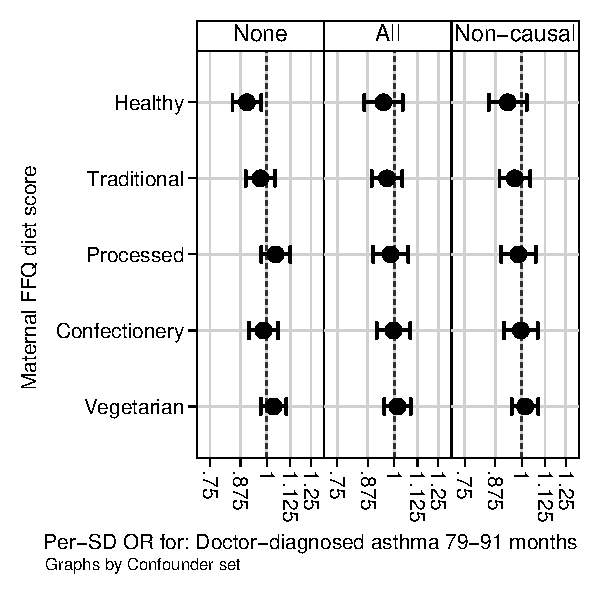
\includegraphics[width=76mm]{figseq1.pdf}
\end{column}
\end{columns}

\end{frame}

\section{Standardization as out--of--sample prediction}

\begin{frame}
\frametitle{Standardization as out--of--sample prediction}

\begin{itemize}

\item<2-> The \texttt{punaf} suite may also be used to compare the \textit{same} scenario between \textit{different} models,
as well as \textit{vice versa}.

\item<3-> For example, we might fit multiple logit models to multiple independent subpopulation datasets,
and then estimate the marginal prevalence that each model would imply in a standard--population dataset,
with a standard distribution of gender and age.

\item<4-> This practice is an example of \textbf{out--of--sample prediction}.

\item<5-> To do this, packages of the \texttt{punaf} suite all have an option \texttt{noesample},
functioning as the option of the same name for \texttt{margins}.

\item<6-> We will illustrate this with an example using \texttt{margprev}.

\end{itemize}

\end{frame}

\begin{frame}
\frametitle{Skin prick allergy prevalences in the GA$^2$LEN Follow--up Survey}

\begin{itemize}

\item<2-> The GA$^2$LEN Follow-up Survey is part of a multi--centre European study on asthma and allergy.

\item<3-> Sensitivity to a number of allergens was measured, using skin prick tests,
in 13 regional subpopulations distributed over Europe.

\item<4-> For each allergen in each subpopulation,
we fitted a logit model of sensitivity to that allergen in that subpopulation,
with respect to age and gender.

\item<5-> The parameters estimated for each such model were then used to estimate the marginal prevalence
expected, if this model applied to a European Standard Population with a standard gender and age distribution.

\item<6-> This was done using \texttt{margprev}, with the \texttt{noesample} option,
in a dataset representing the European Standard Population.

\item<7-> These standardized marginal prevalences were then compared between regional subpopulations,
using a chi--squared heterogeneity test, to detect between--region heterogeneity.

\end{itemize}

\end{frame}

\begin{frame}[fragile]
\frametitle{Logit regression of cat allergy with respect to gender and age in the UK}

In the UK subpopulation, we fitted a logit model of cat allergy
with respect to gender and age,
using sampling--probability weights:

\tiny
\begin{verbatim}
. logit spt_cat male fquesagec [pwei=sampwt5], or

Iteration 0:   log pseudolikelihood = -1030.8768  
Iteration 1:   log pseudolikelihood = -977.80033  
Iteration 2:   log pseudolikelihood = -973.41056  
Iteration 3:   log pseudolikelihood = -973.39866  
Iteration 4:   log pseudolikelihood = -973.39866  

Logistic regression                               Number of obs   =        159
                                                  Wald chi2(2)    =       4.04
                                                  Prob > chi2     =     0.1328
Log pseudolikelihood = -973.39866                 Pseudo R2       =     0.0558

------------------------------------------------------------------------------
             |               Robust
     spt_cat | Odds Ratio   Std. Err.      z    P>|z|     [95% Conf. Interval]
-------------+----------------------------------------------------------------
        male |   2.527963   1.535882     1.53   0.127     .7684525    8.316188
   fquesagec |   .6700974   .2209261    -1.21   0.225     .3511585    1.278712
       _cons |   .0794547   .0300632    -6.69   0.000     .0378487    .1667967
------------------------------------------------------------------------------
\end{verbatim}
\normalsize

The parameter \texttt{\_cons} is the odds of cat allergy in 48--year--old women.
The others are male--gender and per--decade odds ratios.
\textit{However}, not many people understand those parameters. \textit{So$\ldots$}

\end{frame}

\begin{frame}[fragile]
\frametitle{Dataset representing a European Standard Population}

$\ldots$ we now load a dataset with 1 observation per gender per age group,
and data on the gender, the minimum and maximum ages in the age group,
the mean age (uncentered in years and centered at 48 in decades),
and the number in that gender and age group in a European Standard Population:

\tiny
\begin{verbatim}
. use estanpop, clear

. list male agemin agemax agemean fquesagec stanpop, abbr(32) sepby(male)

     +--------------------------------------------------------+
     | male   agemin   agemax   agemean   fquesagec   stanpop |
     |--------------------------------------------------------|
  1. |    0       20       24        22        -2.6      7000 |
  2. |    0       25       29        27        -2.1      7000 |
  3. |    0       30       34        32        -1.6      7000 |
  4. |    0       35       39        37        -1.1      7000 |
  5. |    0       40       44        42         -.6      7000 |
  6. |    0       45       49        47         -.1      7000 |
  7. |    0       50       54        52          .4      7000 |
  8. |    0       55       59        57          .9      6000 |
\end{verbatim}
\normalsize

(Here, we have only showed the younger female age groups.)

\end{frame}

\begin{frame}[fragile]
\frametitle{Cat allergy prevalence standardized to the European Standard Population}

Having loaded the dataset, we now use \texttt{margprev},
with frequency weights and the \texttt{noesample} option,
to estimate the marginal odds and prevalence of cat allergy in the European Standard Population,
using parameters from the model we fitted earlier for the UK:

\tiny
\begin{verbatim}
. margprev [fwei=stanpop], eform noesample
Scenario 1: (asobserved) _all
Confidence interval for the marginal odds
under Scenario 1
Total number of observations used: 134000
------------------------------------------------------------------------------
             |       Odds   Std. Err.      z    P>|z|     [95% Conf. Interval]
-------------+----------------------------------------------------------------
  Scenario_1 |   .1782219     .07486    -4.11   0.000     .0782391    .4059742
------------------------------------------------------------------------------

Asymmetric 95% CI for the untransformed marginal prevalence
under Scenario 1
               Estimate    Minimum    Maximum 
  Scenario_1   .1512635   .0725619   .2887494 
\end{verbatim}
\normalsize

The standardized odds for the UK subpopulation, and for the 12 other regional subpopulations,
were input into the SSC package \texttt{parmhet}
to test for heterogeneity of cat allergy prevalence between European regions.
This heterogeneity was detectable (\textit{I$^2$}=46.4\%, {\textit{P}=.033).

\end{frame}

\section{References}

\begin{frame}
\frametitle{References}

\setbeamerfont{text}{size=\small}

{\scriptsize

\begin{thebibliography}{10}

\bibitem{brady1998}
Brady, A. 1998.
sbe21: Adjusted population attributable fractions from logistic regression.
\textsl{Stata Technical Bulletin} \textbf{42}: 8--12.

\bibitem{greenland1993}
Greenland, S. and K. Drescher.  1993.
Maximum likelihood estimation of the attributable fraction from logistic models.
\textsl{Biometrics} \textbf{49}: 865--872.

\bibitem{hosmer1988}
Hosmer Jr., D. W., S. Lemeshow, and J. Klar.  1988.
Goodness--of--fit testing for the logistic regression model when the estimated probabilities are small.
\textsl{Biometrical Journal} \textbf{30}: 911--924.

\bibitem{newson2013}
Newson, R. B.  2013.
Attributable and unattributable risks and fractions and other scenario comparisons.
\textsl{The Stata Journal} \textbf{13}: 672--698.

\bibitem{shah2004}
Shah, B. V. 2004.
Comment [on Demnati and Rao (2004)].
\textsl{Survey Methodology} \textbf{30}: 29.

\end{thebibliography}

}

\bigskip

The original presentation, and the do--file producing the examples in the birth weight data,
can be downloaded from the conference website at
\href{http://ideas.repec.org/s/boc/usug12.html}{\textsl{http://ideas.repec.org/s/boc/usug12.html}}

\bigskip

The packages
used in this presentation
can be downloaded from SSC, using the \texttt{ssc} command.

\end{frame}

\end{document}
